% You should title the file with a .tex extension (hw1.tex, for example)
\documentclass[11pt]{article}

\usepackage{hyperref}
\usepackage{amsmath}
\usepackage{mathtools}
\usepackage{amssymb}
\usepackage{wrapfig}
\usepackage{fancyhdr}
\usepackage{tikz-qtree}
\usepackage{tikz-qtree-compat}
\usepackage[normalem]{ulem}
\usepackage{tikz}
\usepackage{graphicx}
\DeclareMathOperator*{\argmin}{argmin}
\DeclareMathOperator*{\argmax}{argmax}

\oddsidemargin0cm
\topmargin-2cm     %I recommend adding these three lines to increase the 
\textwidth16.5cm   %amount of usable space on the page (and save trees)
\textheight23.5cm  

\newcommand{\question}[2] {\vspace{.25in} \hrule\vspace{0.5em}
\noindent{\bf #1: #2} \vspace{0.5em}
\hrule \vspace{.10in}}
\renewcommand{\part}[1] {\vspace{.10in} {\bf (#1)}}

\newcommand{\myname}{Sean Bittner}
\newcommand{\myandrew}{srb2201@columbia.edu}
\newcommand{\myhwnum}{12}

\setlength{\parindent}{0pt}
\setlength{\parskip}{5pt plus 1pt}
 
\DeclarePairedDelimiter\abs{\lvert}{\rvert}%
 %
\pagestyle{fancyplain}
\rhead{\fancyplain{}{\myname\\ \myandrew}}

\begin{document}

\medskip                        % Skip a "medium" amount of space
                                % (latex determines what medium is)
                                % Also try: \bigskip, \littleskip

\thispagestyle{plain}
\begin{center}                  % Center the following lines
{\Large Inverting the 5-neuron stomatogastric ganglion (STG) for a distribution of frequencies} \\
Sean Bittner \\
April 21, 2019 \\
\end{center}

\section{Introduction}

Sometimes, you have to give the people what they want.  And, the people have demanded that we DSN the stomatogastric ganglion (STG) of crustaceans.  This was requested by advisers at Woods Hole, the qualification exam committee, and the poster audience at Cosyne.  I have avoided this application in general, due to the perceived intractability of the differentiating through firing frequency measurements in conductance-based biophysical models.  Spending a couple of days taking every possible inch on this problem, it's not too bad, and was actually kind of fun to work on.

\section{STG model}
As suggested by James Fitzgerald, we are analyzing the 5-neuron STG circuit from Gutierrez et al. 2013 \cite{gutierrez2013multiple}.  The STG produces two rhythms in separate parts of the circuit: the fast pyloric rhythm and the slow gastric mill rhythm.  The individual rhythms are often modeled in isolation, but an interesting question is how intermediate neurons interact with the two rhythms, especially when they are strongly electrically coupled to neurons of each rhythm.  In Gutierrez et al. 2013, they set out to study a reduced 5-neuron model of the STG in which two neurons for each rhythm – fast ($f_1$ and $f_2$) and slow ($s_1$ and $s_2$) – interact with an electrically coupled “hub” neuron ($h$).  

\begin{center}
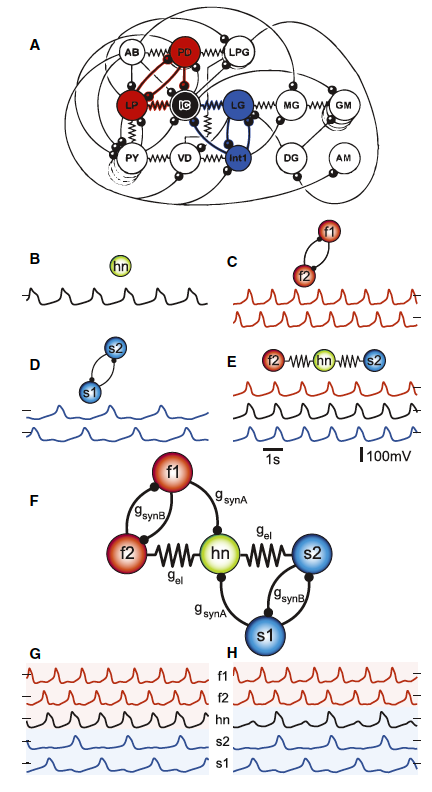
\includegraphics[scale=0.3]{figs/Gutierrez2013_Fig1.png} \\
\end{center}

Check the methods of this paper if you want to see the equations.  It would take a while to write the equations and fixed parameters here.  The paper is focused on how the frequency of the hub neuron changes (locked to fast or low rhythm, or at some intermediate frequency) with respect to three main parameters: $g_{el}$, $g_{synA}$, and $g_{synB}$.

\section{Measuring hub neuron frequency}
In order to measure the frequency of the hub neuron, we must simulate the STG circuit for some number of time steps $T$ and time step $dt$.  We should certainly choose the greatest $dt$ that still gives us accurate circuit behavior.  I determined that to be $dt = 0.025$.  

Our original approach to measuring frequency was to take the max of the fast Fourier transform of the simulated time series.  There are a few key considerations here.  One is resolution in frequency space.  Each FFT entry will correspond to a signal frequency of $\frac{F_s k}{N}$, where N is the number of samples used for the FFT, $F_s = \frac{1}{dt}$, and $k \in \left[0, 1, ..., N-1\right]$.  Our resolution is improved by increasing $N$ and decreasing $dt$.  Increasing N = T-b, where $b$ is some fixed number of buffer burn-in inititaliziation samples, necessitates an increase in simulation time steps $T$, which directly increases computational cost.  Increasing $F_s$ (decreasing $dt$) increases system approximation accuracy, but requires more time steps before a full cycle is observed.  At the level of $dt = 0.025$, thousands of temporal samples were required for resolution of .01Hz.  These challenges in frequency resolution with the discrete Fourier transform motivated the use of an alternative basis of complex exponentials.  Instead, I used a basis of complex exponentials with frequencies from 0.0-1.0 Hz at 0.01Hz resolution.  

Another consideration is that the the frequency spectra of the hub neuron has several peaks.  This is due to high-frequency sub-threshold activity:
\begin{center}
$g_{el} = 6nS$, $g_{synA} = 4nS$, $g_{synB} = 5nS$ \\
\includegraphics[scale=1.0]{figs/v_h_subthreshold.png}
\end{center}
The maximum frequency was often not the firing frequency.  Accordingly, subthreshold activity was set to zero, and the whole signal was low-pass filtered with a moving average window of length 40.  The signal is subsequently mean centered.  After this pre-processing, the maximum frequency in filter bank accurately reflected the firing frequency. (I'll make a nifty signals pic for this eventually).

Now, it takes T = 280, b = 40, to closely replicate Figure 2 from \cite{gutierrez2013multiple}.

\begin{center}
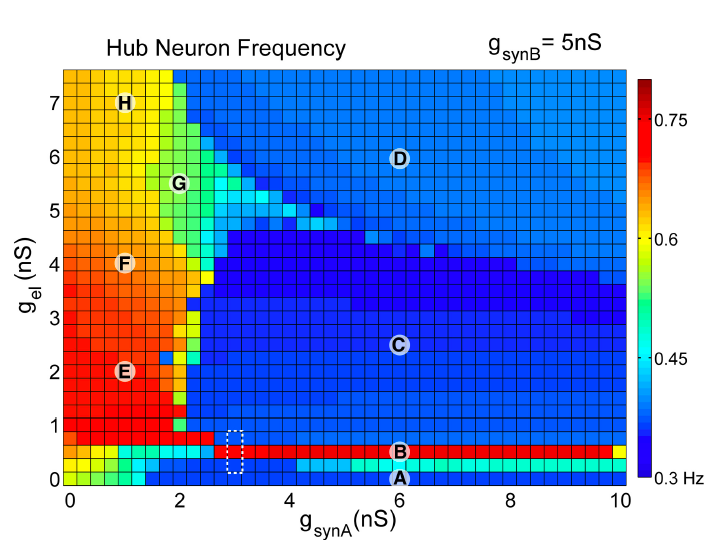
\includegraphics[scale=0.3]{figs/Gutierrez2013_Fig2.png}
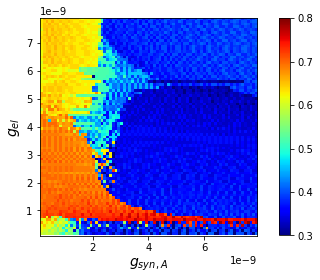
\includegraphics[scale=0.6]{figs/Fig2_rep.png}
\end{center}

A key question is how to differentiate through the maximum frequency identificiation step.  I used a sum-of-powers normalization strategy:

Let $V_h \in \mathcal{C}^N$ be the complex exponential filter bank dot products with the signal $v_h \in \mathcal{R}^N$.  The ``frequency identification" vector is 
\[u = \frac{|V_h|^\alpha}{\sum_{k=1}^N |V_h(k)|^\alpha} \] and the frequencies associated with each element of $V_h$ are $f = \left[ 0.0, 0.01, ..., 1.0 \right]^\top$.

The frequency is then calculated as $f_h = u^\top f$.

\bibliography{dsn}
\bibliographystyle{unsrt}

\end{document}

